\documentclass[ignorenonframetext,]{beamer}

\setbeamertemplate{caption}[numbered]
\setbeamertemplate{caption label separator}{: }
\setbeamercolor{caption name}{fg=normal text.fg}

\beamertemplatenavigationsymbolsempty
\usepackage{lmodern}
\usepackage{amssymb,amsmath}
\usepackage{ifxetex,ifluatex}
\usepackage{fixltx2e} % provides \textsubscript
\ifnum 0\ifxetex 1\fi\ifluatex 1\fi=0 % if pdftex
  \usepackage[T1]{fontenc}
  \usepackage[utf8]{inputenc}
\else % if luatex or xelatex
  \ifxetex
    \usepackage{mathspec}
  \else
    \usepackage{fontspec}
  \fi
  \defaultfontfeatures{Ligatures=TeX,Scale=MatchLowercase}
\fi

% Start adding some content
\usepackage{graphicx}
\usepackage{color}
\usepackage{beamerthemebars}
\usepackage{multicol}
\usepackage{multirow}
\usepackage{hyperref}


\usetheme{Frankfurt}
%%redefined colors for beamer
%\definecolor{beamer@UIUCblue}{RGB}{0,60,125}
%\definecolor{beamer@UIUCorange}{RGB}{244,127,36}
%% taken from
%% http://identitystandards.illinois.edu/graphicstandardsmanual/generalguidelines/colors.html
%
%\definecolor{beamer@UIUCgray}{RGB}{210,210,210}
%\definecolor{beamer@UIUCgray2}{RGB}{244,244,244}
%
%\setbeamercolor{frametitle}{fg=beamer@UIUCblue,bg=beamer@UIUCgray}
%\setbeamercolor{normal text}{fg=black}
%\setbeamercolor{title}{fg=beamer@UIUCblue,bg=beamer@UIUCorange}
%\setbeamercolor{item projected}{fg=white,bg=beamer@UIUCorange}
%
%% Boxes
%\setbeamercolor{block title}{fg=beamer@UIUCblue,bg=beamer@UIUCorange}
%\setbeamercolor{block body}{fg=blue,bg=beamer@UIUCblue!80}
%\setbeamercolor{title in head/foot}{fg=beamer@UIUCblue,bg=beamer@UIUCgray}
%\setbeamercolor{author in head/foot}{fg=white,bg=beamer@UIUCblue}
%\setbeamercolor{institute in head/foot}{fg=white,bg=beamer@UIUCorange}
%\setbeamercolor{date in head/foot}{fg=white,bg=beamer@UIUCorange}
%\setbeamercolor{section in head/foot}{fg=white,bg=beamer@UIUCblue}
%\setbeamercolor{subsection in head/foot}{fg=white,bg=beamer@UIUCorange}
%
%
%\hypersetup{colorlinks=true,urlcolor=beamer@UIUCblue,linkcolor=beamer@UIUCblue,% link color controls section, subsection, and title
%citecolor = beamer@UIUCorange,
%anchorcolor = beamer@UIUCorange}
%
%%override title link color
%\addtobeamertemplate{headline}{\hypersetup{linkcolor=.}}{}
%\addtobeamertemplate{footline}{\hypersetup{linkcolor=.}}{}
%
%% Setup blocks
%\setbeamercolor{block title}{fg = white, bg = beamer@UIUCblue}
%\setbeamercolor{block body}{fg=black,bg=beamer@UIUCgray2}
%
%\setbeamercolor{block title alerted}{fg = white, bg = beamer@UIUCorange}
%\setbeamercolor{block body alerted}{fg=black,bg=beamer@UIUCgray2}
%
%\setbeamercolor{block title example}{fg = beamer@UIUCblue, bg = beamer@UIUCgray}
%\setbeamercolor{block body example}{fg=black,bg=beamer@UIUCgray2}

% use upquote if available, for straight quotes in verbatim environments
\IfFileExists{upquote.sty}{\usepackage{upquote}}{}
% use microtype if available
\IfFileExists{microtype.sty}{%
\usepackage{microtype}
\UseMicrotypeSet[protrusion]{basicmath} % disable protrusion for tt fonts
}{}
\newif\ifbibliography
\usepackage{graphicx,grffile}
\makeatletter
\def\maxwidth{\ifdim\Gin@nat@width>\linewidth\linewidth\else\Gin@nat@width\fi}
\def\maxheight{\ifdim\Gin@nat@height>\textheight0.8\textheight\else\Gin@nat@height\fi}
\makeatother
% Scale images if necessary, so that they will not overflow the page
% margins by default, and it is still possible to overwrite the defaults
% using explicit options in \includegraphics[width, height, ...]{}
\setkeys{Gin}{width=\maxwidth,height=\maxheight,keepaspectratio}

% Prevent slide breaks in the middle of a paragraph:
\widowpenalties 1 10000
\raggedbottom


\setlength{\parindent}{0pt}
\setlength{\parskip}{6pt plus 2pt minus 1pt}
\setlength{\emergencystretch}{3em}  % prevent overfull lines
\providecommand{\tightlist}{%
  \setlength{\itemsep}{0pt}\setlength{\parskip}{0pt}}
\setcounter{secnumdepth}{0}
\usepackage{amsmath, bbm, graphicx}


\author[
Xuelong Wang
]{Xuelong Wang}
\date[
01/08/2018
]{
January 08, 2018
}

% Option to fake out the raw_tex plugin and, thus, enabling the embedding of
% markdown within a column scheme.
% See:
% (1) https://groups.google.com/forum/#!msg/pandoc-discuss/vcy7v9Uk95U/LDgWJTHTRR4J
% (2) http://stackoverflow.com/questions/15142134/slides-with-columns-in-pandoc
\def\begincols{\begin{columns}}
\def\endcols{\end{columns}}

\begin{document}

% Necessary due to the ignorenonframetext requirement
% See: http://tex.stackexchange.com/questions/181032/ignorenonframetext-option-breaks-frame-background-color-option
\mode<all>{
\title[
SIR
]{
%\begin{columns}
%\column{.25\textwidth}
%\hspace{.2in}
%\vspace{.1in}
%\includegraphics{ilogo.pdf}
%\column{.85\textwidth}
Sliced Inverse Regression For Dimension Reduction (Ker-Chau Li)
%\end{columns}
}
}
\mode*

\frame{\titlepage}

\begin{frame}
\tableofcontents[hideallsubsections]
\end{frame}

\section{Introduction}\label{introduction}

\subsection{Introduction}\label{introduction-1}

\begin{frame}{Regression Anlysis}

\begin{itemize}
\tightlist
\item
  Study the relationship of a response variable y and its explanatory
  variable x
\item
  Parametric model\\
\item
  e.g.~Linear Regression\\
\item
  Nonparametric model\\
\item
  e.g.~Locall smoothing
\end{itemize}

\end{frame}

\begin{frame}{Curse of Dimensionality}

\begin{itemize}
\tightlist
\item
  When the dimension of x gets higher, the number of observation gets
  much smaller
\item
  Standard methods probably will break down due to the sparseness of
  data
\item
  We need to reduce the dimemsion of x so that it's easier for
  visualized data and fitting model
\end{itemize}

\end{frame}

\section{Model}\label{model}

\subsection{Model}\label{model-1}

\begin{frame}{Model}

\begin{block}{Model Settings}
\[
  y = f(\beta_1x, \dots, \beta_kx, \epsilon),
\]
$x$ is explanatory variable, column vectors on $R^p$,\\   
$\beta's$ is unknown row vectors, \\
$\epsilon$ is independent of $x$, \\
$f$ is an arbitrary unkonw function on $R^{p+1}$ \\
\end{block}

\[ (\beta_1x, \dots, \beta_kx)' \]

\begin{itemize}
\tightlist
\item
  Projection of the \(x\in R^p\) into \(R^k\), we assume that k is much
  smaller than p
\item
  Captures all we need to know about y
\end{itemize}

\end{frame}

\begin{frame}{Model}

\begin{block}{Effective dimension-reduction}
Effective dimension-reduction directions (e.d.r) : any linear combination of $\beta's$ \\
$B = Span(\beta)$: The linear space spaned by $\beta's$\\
\end{block}

Note: Since \(f\) is arbitrary, only the \(B\) can be identified

\begin{itemize}
\tightlist
\item
  Inverse Regression one of the methods of estimating the Effective
  dimension-reduction directions
\end{itemize}

\end{frame}

\section{Inverse Regression}\label{inverse-regression}

\subsection{Inverse Regression}\label{inverse-regression-1}

\begin{frame}{Inverse Regression}

\begin{block}{Inverse Regression}

\begin{itemize}
\tightlist
\item
  Regress x against of y
\item
  From one p-dimenstion problem to p One-dimenstion regression problems
\end{itemize}

\end{block}

\end{frame}

\begin{frame}{Inverse Regression Curve}

\begin{block}{Inverse Regression Curve}

\[
  E(x|y) \in R^p
\] is a curve as y varies, \[
  E(E(x|y)) = E(x)
\] is the center of \(E(x|y)\),

\[ E(x|y) - E(x)\] is the centered inverse regression curve

\begin{itemize}
\tightlist
\item
  With certain conditions, the centred inverse curve is related with the
  e.d.r.
\end{itemize}

\end{block}

\end{frame}

\begin{frame}{Inverse Regression}

\begin{block}{Assumption}

\[
  y = f(\beta_1x, \dots, \beta_kx, \epsilon), \Leftrightarrow y|\beta indepndent x  
\]

\end{block}

\begin{block}{Condition 3.1}

For any \(b\) in \(R^p\),
\[E(bx|\beta_1x, \dots, \beta_kx) = c_0 + c_1\beta_1x, \dots, c_k\beta_kx\]

\end{block}

\end{frame}

\begin{frame}{e.d.r and Inverser Regression Curve}

\begin{block}{Theorem 3.1} 
Under the previous Conditions,
\[ E(x|y) - E(x) \subset Span(\beta_k\Sigma_{xx}),k = 1, \dots, K\]
The centered inverse regression curve is contained in the linear subsapce spannned by $\beta_k\Sigma_{xx}$
\end{block}

\end{frame}

\begin{frame}{e.d.r and Inverser Regression Curve}

\begin{block}{Corollary 3.1} 
\[ z = \Sigma_{xx}^{-1/2}[x-E(x)] \]
x is the standardized 

\[ f(\beta_1x, \dots, \beta_kx, \epsilon) \Rightarrow f(\eta_1x, \dots, \eta_kx, \epsilon) \Rightarrow \beta_k = \eta_k \Sigma_{xx}^{-1/2}\]

\[E(z|y) - E(z) \subset Span(\eta_k), k=1 ,\dots, K\]
\end{block}

\end{frame}

\begin{frame}{An Important consequence}

\begin{itemize}
\tightlist
\item
  The covariance matrix \(cov(E(z|y))\) is degenerate in any direction
  which is orthogonal to the \(\eta's\)
\item
  \({\eta_k}^{'}s( k =1, \dots, K)\) associated with largest K
  eigenvalues of \(cov(E(z|y))\)
\end{itemize}

\begin{block}{How to estimate the \(cov(E(z|y))\)}

That leads to Sliced Inverse Regression Method

\end{block}

\end{frame}

\section{Sliced Inverse Regression
Method}\label{sliced-inverse-regression-method}

\subsection{Sliced Inverse Regression
Method}\label{sliced-inverse-regression-method-1}

\begin{frame}{Sliced Inverse Regression Method}

\begin{enumerate}
\def\labelenumi{\arabic{enumi}.}
\tightlist
\item
  Standardize x

  \begin{itemize}
  \tightlist
  \item
    \(z_i = \Sigma_{xx}^{-1/2}(x_i - \bar{x})(i = 1, \dots, n)\)
  \end{itemize}
\item
  Divide the range of y into H slices, \(I_1, \dots , I_H\)

  \begin{itemize}
  \tightlist
  \item
    \(\hat{p}_h = (1/n)\sum_{i=1}^n(I_{y_i\in I_h})\)
  \end{itemize}
\item
  Calcuate the sample mean for each slice

  \begin{itemize}
  \tightlist
  \item
    \(\hat{m}_h = (1/n\hat{p}_h) \sum_{y_i \in I_h}z_i\)
  \end{itemize}
\item
  Conduct a (weighted) principle component analysis on covariance matrix

  \begin{itemize}
  \tightlist
  \item
    \(\hat{V} = \sum_{h=1}^{H} \hat{p}_h\hat{m}_h\hat{m}_h'\)
  \end{itemize}
\item
  Select the K largest eigenvectors (row vectors)

  \begin{itemize}
  \tightlist
  \item
    \(\hat{\eta}_k (k = 1, ... , K)\)
  \end{itemize}
\item
  Transform the eigenvectors back to original scale

  \begin{itemize}
  \tightlist
  \item
    \(\hat{\beta}_k = \hat{\eta}_k \hat{\Sigma}_{xx}^{-1/2}\)
  \end{itemize}
\end{enumerate}

\end{frame}

\section{Simulation}\label{simulation}

\subsection{Simulation}\label{simulation-1}

\begin{frame}{Simulation 1}

\begin{exampleblock}{Simulation settings}
\begin{align*}
y &= x_1 + x_2 + x_3 + x_4 + 0x_5 + \epsilon 
\end{align*}
\begin{itemize}
    \item $n = 100$
    \item Only one component $\beta = (1,1,1,1,0)$
    \item Normalized target $\beta^* = (0.5, 0.5, 0.5, 0.5, 0)$
    \item The number of slice $H = (5, 10, 20)$
\end{itemize}
\end{exampleblock}

\end{frame}

\begin{frame}{Simulation 1 results}

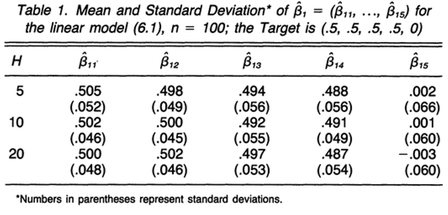
\includegraphics[height=0.1]{./pic/result_1} - Repeat the simulation 100
times to generate the emprical distribution of \(\beta's\)

\end{frame}

\begin{frame}{Simulation 2}

\begin{exampleblock}{Simulation settings}
\begin{align*}
y &= x_1(x_1 + x_2 + 1) + \sigma \cdot \epsilon \\
y &= \frac{x_1}{0.5 + {(x_2 + 1.5)}^2} + \sigma \cdot \epsilon
\end{align*}
\begin{itemize}
    \item $n = 400$
    \item $\sigma = (0.5, ~1) $
    \item The number of slice $H = (5, 10, 20)$ 
    \item Two component $\beta_1 = (1,0,0,0,0), ~ \beta_2 = (0,1,0,0,0)$
\end{itemize}
\end{exampleblock}

\end{frame}

\begin{frame}{Simulation 1 results}

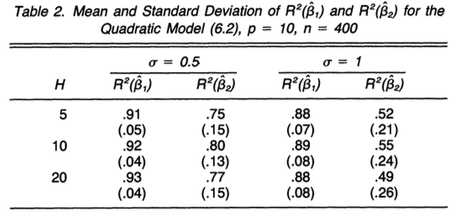
\includegraphics{./pic/result_2.png}
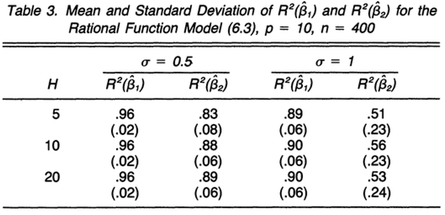
\includegraphics{./pic/result_3.png}

\begin{itemize}
\tightlist
\item
  Repeat the simulation 100 times to generate the emprical distribution
  of \(\beta's\)
\end{itemize}

\end{frame}

\begin{frame}{}

\begin{center}
\Huge Thank you
\end{center}

\end{frame}

\begin{frame}{Reference}

\hypertarget{refs}{}
\hypertarget{ref-ref5}{}
Tonglin Zhang, Baijian Yang. 2016. ``Big Data Dimension Reduction Using
Pca.''

\end{frame}

\end{document}
